%=================================================================
% CSE 4345 — Big Data Analytics
% Week 4, Part 1: The Key-Value Paradigm —
%                 MapReduce, Pig, Hive, and HBase
% Department of CSE, Premier University
%
% Part 1 covers: MapReduce model (Map · Shuffle/Sort · Combine · Reduce)
%               · Execution pipeline · Fault tolerance · Pig dataflow
%               · Hive SQL-on-Hadoop · HBase column-family NoSQL
%               · Ecosystem tool selection · Ivy League alignment · Assessment
% Part 2 covers: Dean & Ghemawat (2004) · Bigtable (Chang 2006) · Facebook Hive case
%=================================================================

\documentclass[aspectratio=169,10pt]{beamer}

%---------- Packages ----------
\usepackage[utf8]{inputenc}
\usepackage[T1]{fontenc}
\usepackage{booktabs}
\usepackage{xcolor}
\usepackage{tikz}
\usetikzlibrary{shapes.geometric, positioning, arrows.meta,
                decorations.pathreplacing, calc, fit, backgrounds, matrix}
\usepackage{amsmath}
\usepackage{graphicx}
\usepackage{multicol}
\usepackage{enumerate}
\usepackage{array}
\usepackage{listings}

%---------- Theme ----------
\usetheme{Madrid}

%---------- Premier University Color Identity ----------
\definecolor{PUNavy}{RGB}{10,36,99}
\definecolor{PUGold}{RGB}{197,151,37}
\definecolor{PULightBlue}{RGB}{210,228,255}
\definecolor{PUTeal}{RGB}{0,100,100}
\definecolor{PUGray}{RGB}{90,90,90}
\definecolor{PURed}{RGB}{160,30,30}
\definecolor{PUGreen}{RGB}{30,120,60}
\definecolor{PUOrange}{RGB}{200,100,20}
\definecolor{PUPurple}{RGB}{80,0,120}

\setbeamercolor{palette primary}{bg=PUNavy, fg=white}
\setbeamercolor{palette secondary}{bg=PUNavy!85, fg=white}
\setbeamercolor{palette tertiary}{bg=PUNavy!70, fg=white}
\setbeamercolor{palette quaternary}{bg=PUNavy, fg=white}
\setbeamercolor{structure}{fg=PUNavy}
\setbeamercolor{title}{bg=PUNavy, fg=PUGold}
\setbeamercolor{subtitle}{fg=white}
\setbeamercolor{frametitle}{bg=PUNavy, fg=PUGold}
\setbeamercolor{alerted text}{fg=PUGold!85!black}
\setbeamercolor{block title}{bg=PUNavy, fg=white}
\setbeamercolor{block body}{bg=PULightBlue!45}
\setbeamercolor{block title alerted}{bg=PUGold!80!black, fg=white}
\setbeamercolor{block body alerted}{bg=PUGold!12}
\setbeamercolor{block title example}{bg=PUTeal, fg=white}
\setbeamercolor{block body example}{bg=PUTeal!10}
\setbeamercolor{section in toc}{fg=PUNavy}
\setbeamercolor{itemize item}{fg=PUGold!80!black}
\setbeamercolor{itemize subitem}{fg=PUNavy!70}

\setbeamertemplate{navigation symbols}{}
\setbeamertemplate{itemize item}{\scriptsize\raise1.5pt\hbox{\textbullet}}
\setbeamertemplate{itemize subitem}{\scriptsize\raise1pt\hbox{--}}

%---------- Code listing style ----------
\lstset{
  basicstyle=\ttfamily\scriptsize,
  backgroundcolor=\color{PUNavy!8},
  frame=single,
  rulecolor=\color{PUNavy!30},
  breaklines=true,
  keywordstyle=\color{PUNavy}\bfseries,
  commentstyle=\color{PUGray}\itshape,
  stringstyle=\color{PUGreen!70!black},
}

%---------- Section separator ----------
\AtBeginSection[]{
  \begin{frame}[plain]
    \vfill
    \centering
    \begin{beamercolorbox}[sep=12pt,center,shadow=true,rounded=true]{block title}
      \usebeamerfont{title}\insertsectionhead\par
    \end{beamercolorbox}
    \vfill
  \end{frame}
}

%---------- Title metadata ----------
\title[CSE 4345 \textbar{} Week 4, Part 1]{CSE 4345: Big Data Analytics}
\subtitle{Week 4, Part 1 \textemdash\ The Key-Value Paradigm:
          MapReduce, Pig, Hive \& HBase}
\author[Dept.\ of CSE]{Department of Computer Science \& Engineering\\[4pt]
       \small Premier University, Chittagong}
\institute{}
\date{Semester 2026}

%=================================================================
\begin{document}
%=================================================================

%----------------------------------------------------------------
% TITLE SLIDE
%----------------------------------------------------------------
\begin{frame}
  \titlepage
\end{frame}

%----------------------------------------------------------------
% COURSE INFO
%----------------------------------------------------------------
\begin{frame}{Course \& Lecture Information}
  \begin{columns}[T]
    \column{0.47\textwidth}
      \begin{block}{Lecture Identity}
        \begin{tabular}{ll}
          \textbf{Course:}      & CSE 4345 \\
          \textbf{Week / Part:} & 4 of 11 \textbar\ Part 1 of 2 \\
          \textbf{CLO:}         & CLO1 \\
          \textbf{PLO:}         & PLO(a) \\
        \end{tabular}
      \end{block}
      \vspace{6pt}
      \begin{alertblock}{CLO1}
        \textit{``Understand big data characteristics and the technologies used to process them''}
      \end{alertblock}
      \vspace{6pt}
      \begin{block}{Course Progression}
        \small
        Week 2: Data integration challenges\\
        Week 3: Where data lives (HDFS)\\
        \textbf{Week 4: How data is \emph{processed} (MapReduce + tools)}\\
        Week 5: File formats, YARN, optimisation
      \end{block}

    \column{0.50\textwidth}
      \begin{exampleblock}{Part 1 Covers}
        \begin{itemize}
          \item Why we need a new computation model for HDFS
          \item The MapReduce programming model (Map · Shuffle/Sort · Reduce)
          \item The Combiner: local mini-reducer optimisation
          \item The Partitioner: directing keys to Reducers
          \item Full MapReduce execution pipeline with fault tolerance
          \item Apache Pig: dataflow scripting (Pig Latin)
          \item Apache Hive: SQL-on-Hadoop (HiveQL)
          \item Apache HBase: column-family NoSQL on Hadoop
          \item Ecosystem tool selection matrix
          \item Ivy League alignment
          \item Student assessment pool
        \end{itemize}
      \end{exampleblock}
  \end{columns}
\end{frame}

%----------------------------------------------------------------
% AGENDA
%----------------------------------------------------------------
\begin{frame}{Lecture Agenda}
  \tableofcontents
\end{frame}

%================================================================
\section{Why a New Computation Model?}
%================================================================

\begin{frame}{The Computation Problem on Distributed Storage}
  \begin{columns}[T]
    \column{0.52\textwidth}
      \begin{block}{The Challenge (2003)}
        Google has petabytes of web crawl data on a 1{,}000-node GFS cluster.  To build a search index, they need to:
        \begin{itemize}
          \item Process every document (sequential scan over petabytes)
          \item Aggregate data by key (e.g., group URLs by domain)
          \item Do this \textbf{fast}: a single thread processes $\sim$100 MB/s; a petabyte takes $>$2.7 hours per pass even at full disk speed
          \item \textbf{Tolerate failures}: any node can fail mid-job; the job must still complete
        \end{itemize}
      \end{block}
      \vspace{4pt}
      \begin{alertblock}{The SQL Answer is Wrong Here}
        Traditional SQL requires data in a \textbf{relational schema}, supports \textbf{random access}, and runs on a \textbf{single server}.  None of these properties hold for unstructured petabyte data on HDFS.
      \end{alertblock}

    \column{0.45\textwidth}
      \begin{exampleblock}{The Key Insight (Dean \& Ghemawat, 2004)}
        \large\centering
        \vspace{4pt}
        \textbf{Every large-scale computation can be expressed as:}
        \vspace{8pt}
        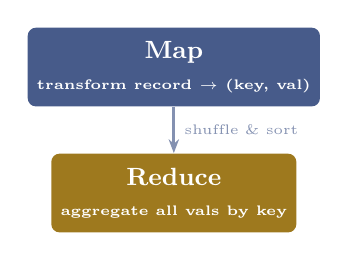
\begin{tikzpicture}[
            box/.style={rectangle, rounded corners=3pt, minimum width=2.8cm,
                        minimum height=1.0cm, align=center, font=\small\bfseries}
          ]
          \node[box, fill=PUNavy!75, text=white] (m) at (0, 0)
                {Map\\{\tiny transform record $\to$ (key, val)}};
          \node[box, fill=PUGold!80!black, text=white] (r) at (0,-1.6)
                {Reduce\\{\tiny aggregate all vals by key}};
          \draw[-{Stealth[length=5pt]}, very thick, PUNavy!50]
                (m) -- node[right, font=\tiny]{shuffle \& sort} (r);
        \end{tikzpicture}
        \vspace{8pt}
        \textit{``If you can write it as Map + Reduce, the framework parallelises it automatically across 1{,}000 machines.''}
      \end{exampleblock}
  \end{columns}
\end{frame}

%================================================================
\section{The MapReduce Programming Model}
%================================================================

\begin{frame}[fragile]{MapReduce: The Word Count Canonical Example}
  \begin{columns}[T]
    \column{0.50\textwidth}
      \begin{block}{Problem}
        Count the frequency of every word in a multi-terabyte document collection.
      \end{block}
      \vspace{4pt}
      \begin{exampleblock}{Step-by-Step Execution}
        \textbf{Input split (one per Mapper):}\\
        \texttt{\small "the cat sat on the mat"}
        \vspace{4pt}
        \textbf{Map phase} — emit (word, 1) for each word:
        \begin{center}
        \texttt{\scriptsize (the,1) (cat,1) (sat,1) (on,1) (the,1) (mat,1)}
        \end{center}
        \textbf{Shuffle \& Sort} — group by key:
        \begin{center}
        \texttt{\scriptsize (cat,[1]) (mat,[1]) (on,[1]) (sat,[1]) (the,[1,1])}
        \end{center}
        \textbf{Reduce phase} — sum each list:
        \begin{center}
        \texttt{\scriptsize (cat,1) (mat,1) (on,1) (sat,1) (the,2)}
        \end{center}
      \end{exampleblock}

    \column{0.47\textwidth}
      \begin{alertblock}{Formal Definition} 
        \textbf{Map:} $(k_1, v_1) \;\to\; \text{list}(k_2, v_2)$\\
        \textbf{Reduce:} $(k_2, \text{list}(v_2)) \;\to\; \text{list}(v_3)$\\[4pt]
        Both functions are \textbf{user-defined}; the framework handles everything else: data distribution, task scheduling, progress tracking, and failure recovery.
      \end{alertblock}
      \vspace{4pt}
      \begin{block}{Mapper Pseudocode}
        \begin{lstlisting}[language=Python]
def map(key, value):
    # value = one line of text
    for word in value.split():
        emit(word, 1)
        \end{lstlisting}
      \end{block}
      \begin{block}{Reducer Pseudocode}
        \begin{lstlisting}[language=Python]
def reduce(key, values):
    # key = word, values = [1,1,1,...]
    emit(key, sum(values))
        \end{lstlisting}
      \end{block}
  \end{columns}
\end{frame}

%----------------------------------------------------------------
\begin{frame}{MapReduce Execution Pipeline}
  \begin{center}
  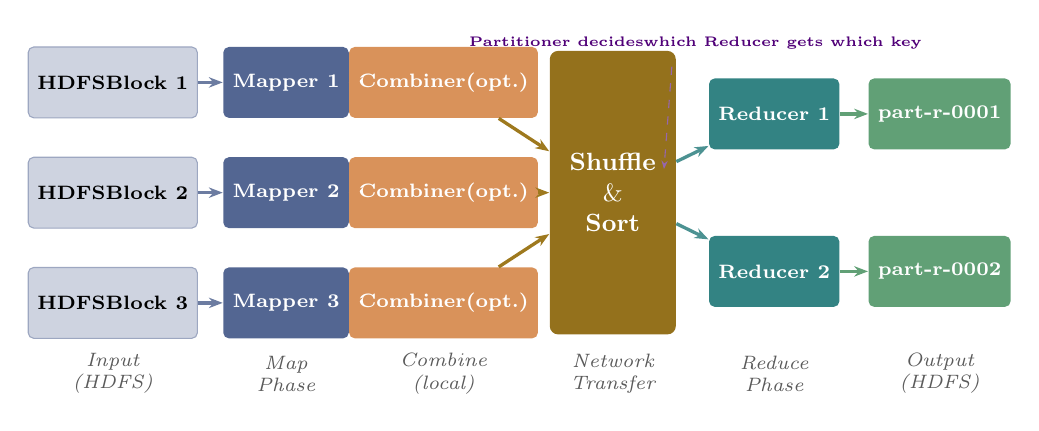
\begin{tikzpicture}[
      phase/.style={rectangle, rounded corners=3pt, draw=PUNavy!40,
                    minimum width=1.8cm, minimum height=2.4cm,
                    align=center, font=\small\bfseries},
      arr/.style={-{Stealth[length=5pt]}, very thick, PUNavy!60},
      lbl/.style={font=\scriptsize\itshape, PUGray, align=center}
    ]
    % Input blocks (HDFS)
    \foreach \i/\y in {1/2.0, 2/0.6, 3/-0.8} {
      \node[rectangle, fill=PUNavy!20, draw=PUNavy!40, rounded corners=2pt,
            minimum width=1.6cm, minimum height=0.9cm,
            font=\scriptsize\bfseries]
            (blk\i) at (-5.5, \y) {HDFS\\Block \i};
    }
    \node[lbl] at (-5.5,-1.7) {Input\\(HDFS)};

    % Mappers
    \foreach \i/\y in {1/2.0, 2/0.6, 3/-0.8} {
      \node[rectangle, fill=PUNavy!70, text=white,
            rounded corners=2pt, minimum width=1.5cm, minimum height=0.9cm,
            font=\scriptsize\bfseries]
            (map\i) at (-3.3, \y) {Mapper \i};
      \draw[arr] (blk\i) -- (map\i);
    }
    \node[lbl] at (-3.3,-1.7) {Map\\Phase};

    % Combiners (optional)
    \foreach \i/\y in {1/2.0, 2/0.6, 3/-0.8} {
      \node[rectangle, fill=PUOrange!70, text=white,
            rounded corners=2pt, minimum width=1.4cm, minimum height=0.9cm,
            font=\scriptsize\bfseries]
            (comb\i) at (-1.3, \y) {Combiner\\(opt.)};
      \draw[arr, PUOrange!70] (map\i) -- (comb\i);
    }
    \node[lbl] at (-1.3,-1.7) {Combine\\(local)};

    % Shuffle & Sort (abstract)
    \node[rectangle, fill=PUGold!75!black, text=white, rounded corners=3pt,
          minimum width=1.6cm, minimum height=3.6cm,
          font=\small\bfseries, align=center]
          (shuf) at (0.85, 0.6) {Shuffle\\$\&$\\Sort};
    \foreach \i in {1,2,3} {
      \draw[arr, PUGold!80!black] (comb\i) -- (shuf);
    }
    \node[lbl] at (0.85,-1.7) {Network\\Transfer};

    % Reducers
    \foreach \i/\y in {1/1.6, 2/-0.4} {
      \node[rectangle, fill=PUTeal!80, text=white,
            rounded corners=2pt, minimum width=1.5cm, minimum height=0.9cm,
            font=\scriptsize\bfseries]
            (red\i) at (2.9, \y) {Reducer \i};
      \draw[arr, PUTeal!70] (shuf) -- (red\i);
    }
    \node[lbl] at (2.9,-1.7) {Reduce\\Phase};

    % Output (HDFS)
    \foreach \i/\y in {1/1.6, 2/-0.4} {
      \node[rectangle, fill=PUGreen!70, text=white,
            rounded corners=2pt, minimum width=1.6cm, minimum height=0.9cm,
            font=\scriptsize\bfseries]
            (out\i) at (5.0, \y) {part-r-000\i};
      \draw[arr, PUGreen!70] (red\i) -- (out\i);
    }
    \node[lbl] at (5.0,-1.7) {Output\\(HDFS)};

    % Partitioner label
    \node[font=\tiny\bfseries, PUPurple] at (1.9, 2.5)
          {Partitioner decides\\which Reducer gets which key};
    \draw[-{Stealth[length=3pt]}, PUPurple!60, thin, dashed]
          (1.6,2.2) -- (1.5,0.9);
  \end{tikzpicture}
  \end{center}
  \vspace{2pt}
  \begin{alertblock}{The Shuffle is the Bottleneck}
    The shuffle phase transfers intermediate data \textbf{across the network}.  Minimizing shuffle volume is the primary MapReduce performance optimisation.  The \textbf{Combiner} reduces shuffle traffic by pre-aggregating locally.
  \end{alertblock}
\end{frame}

%----------------------------------------------------------------
\begin{frame}[fragile]{The Combiner: Local Mini-Reducer}
  \begin{columns}[T]
    \column{0.50\textwidth}
      \begin{block}{Why the Combiner Exists}
        In word count, each Mapper emits $(the, 1)$ for every occurrence of ``the'' in its input split.  If a split contains 10{,}000 occurrences of ``the'', the Mapper emits 10{,}000 pairs, each sent over the network during shuffle.
        \vspace{4pt}

        With a \textbf{Combiner} running on the Mapper's output \emph{before} network transfer:
        \begin{itemize}
          \item Locally sum all $(the, 1)$ pairs $\to$ emit $(the, 10000)$
          \item \textbf{Network traffic reduced by $\sim$10{,}000$\times$} for this key
        \end{itemize}
      \end{block}
      \vspace{4pt}
      \begin{alertblock}{Combiner Constraint}
        The Combiner must have the \textbf{same input and output types} as the Reducer, and the operation must be \textbf{associative and commutative} (e.g., sum, min, max, count).  It \alert{cannot} be used for non-associative operations like average or median.
      \end{alertblock}

    \column{0.47\textwidth}
      \begin{exampleblock}{Without vs.\ With Combiner}
        \textbf{Without:}
        \begin{itemize}
          \small
          \item Mapper output: \texttt{(the,1)} $\times$ 10{,}000 pairs
          \item Network send: 10{,}000 records per key
        \end{itemize}
        \vspace{6pt}
        \textbf{With Combiner:}
        \begin{itemize}
          \small
          \item Mapper output: \texttt{(the,1)} $\times$ 10{,}000
          \item Combiner locally: \texttt{(the,10000)} — 1 record
          \item Network send: \textbf{1 record per key}
        \end{itemize}
        \vspace{6pt}
        \begin{lstlisting}[language=Java, title={Java: Setting Combiner}]
Job job = Job.getInstance(conf);
job.setMapperClass(WordMapper.class);
// Combiner class = Reducer class
job.setCombinerClass(SumReducer.class);
job.setReducerClass(SumReducer.class);
        \end{lstlisting}
      \end{exampleblock}
  \end{columns}
\end{frame}

%----------------------------------------------------------------
\begin{frame}{MapReduce Fault Tolerance}
  \begin{columns}[T]
    \column{0.52\textwidth}
      \begin{block}{How MapReduce Handles Node Failure}
        The \textbf{ApplicationMaster} (YARN) monitors every task.  If a node fails:
        \vspace{4pt}
        \begin{enumerate}
          \item ApplicationMaster detects missing heartbeat ($>$10 minutes = task dead)
          \item \textbf{Failed Map tasks} are re-scheduled on any available node (input data still in HDFS)
          \item \textbf{Failed Reduce tasks} are re-scheduled; must re-read shuffle data
          \item \textbf{Speculative execution}: if a task is unusually slow, run a duplicate on another node — accept the first to finish, kill the other (``straggler mitigation'')
        \end{enumerate}
      \end{block}
      \vspace{4pt}
      \begin{exampleblock}{Why Re-execution Works}
        Map functions are \textbf{pure} (no side effects, no shared state between tasks).  Given the same input block, a re-executed Mapper always produces the same intermediate output.  This \emph{idempotency} is what makes fault recovery cheap.
      \end{exampleblock}

    \column{0.45\textwidth}
      \begin{alertblock}{Bangladesh Context: Pathao Ride Analytics}
        \textbf{Scenario:} Pathao processes $\sim$500{,}000 completed rides per day.  Each ride record (JSON, $\sim$2 KB) contains: rider ID, driver ID, start/end coordinates, distance, fare, timestamp.
        \vspace{4pt}
        \textbf{MapReduce jobs run nightly:}
        \begin{itemize}
          \small
          \item Mapper: emit \texttt{(driver\_id, fare)}
          \item Reducer: compute driver earnings per day
          \item Combiner: pre-sum fares within each Mapper's split
        \end{itemize}
        \textbf{Scale:} $\sim$1 GB/day; runs across 10 nodes in $<$3 min.  During a node crash mid-job, the failed Mapper tasks re-execute on healthy nodes; the job still completes.
      \end{alertblock}
  \end{columns}
\end{frame}

%================================================================
\section{Apache Pig: Dataflow Scripting}
%================================================================

\begin{frame}[fragile]{Apache Pig: ETL in Pig Latin}
  \begin{columns}[T]
    \column{0.50\textwidth}
      \begin{block}{What is Pig?}
        Apache Pig is a \textbf{high-level dataflow scripting platform} that compiles a scripting language called \textbf{Pig Latin} into MapReduce jobs automatically.  Designed for data engineers who need to build complex ETL pipelines without writing Java.
        \vspace{4pt}
        \begin{itemize}
          \item \textbf{Procedural}: expresses \emph{how} data flows step-by-step
          \item Each statement defines a transformation on a \textbf{relation} (bag of tuples)
          \item Optimizer rewrites the script into an efficient MapReduce DAG
          \item Extensible: custom UDFs in Java, Python, or Ruby
        \end{itemize}
      \end{block}
      \vspace{4pt}
      \begin{alertblock}{When to Use Pig}
        \begin{itemize}
          \small
          \item Complex multi-step ETL pipelines with joins, filters, and aggregations
          \item Semi-structured or nested data (JSON, Avro) that doesn't map to a flat table easily
          \item When the data analyst prefers a scripting mental model over SQL
        \end{itemize}
      \end{alertblock}

    \column{0.47\textwidth}
      \begin{exampleblock}{Pig Latin: bKash Transaction Example}
        \begin{lstlisting}[language={},
            title={Find top-5 merchants by total revenue}]
-- Load raw transactions from HDFS
txns = LOAD '/data/bkash/txns'
       USING PigStorage(',')
       AS (txn_id:chararray,
           merchant:chararray,
           amount:float,
           status:chararray,
           dt:chararray);

-- Filter: only completed payments
paid = FILTER txns
       BY status == 'COMPLETED';

-- Group by merchant
grp = GROUP paid BY merchant;

-- Sum revenue per merchant
rev = FOREACH grp GENERATE
      group         AS merchant,
      SUM(paid.amount) AS revenue;

-- Sort descending
ranked = ORDER rev
         BY revenue DESC;

-- Take top 5
top5 = LIMIT ranked 5;

DUMP top5;
        \end{lstlisting}
      \end{exampleblock}
  \end{columns}
\end{frame}

%================================================================
\section{Apache Hive: SQL on Hadoop}
%================================================================

\begin{frame}{Apache Hive: HiveQL and the Metastore}
  \begin{columns}[T]
    \column{0.50\textwidth}
      \begin{block}{What is Hive?}
        Apache Hive provides a \textbf{data warehousing layer on top of HDFS}, exposing a SQL dialect called \textbf{HiveQL} that is compiled into MapReduce, Tez, or Spark jobs at runtime.  Data analysts write SQL; the cluster does the rest.
      \end{block}
      \vspace{4pt}
      \begin{exampleblock}{Hive Architecture}
        \begin{center}
        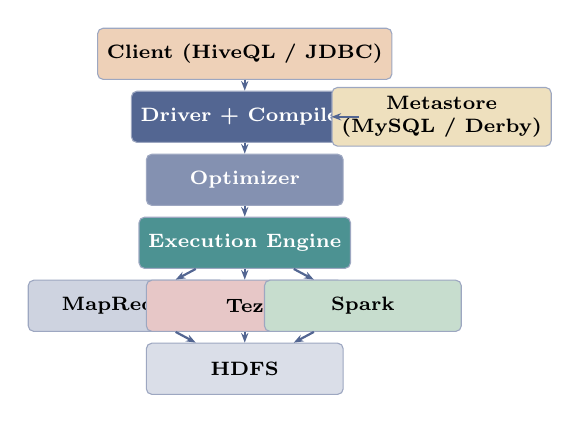
\begin{tikzpicture}[
            box/.style={rectangle, rounded corners=2pt, draw=PUNavy!40,
                        minimum width=2.5cm, minimum height=0.65cm,
                        font=\scriptsize\bfseries, align=center},
            arr/.style={-{Stealth[length=3.5pt]}, PUNavy!70, thick}
          ]
          \node[box, fill=PUOrange!30]  (cli)  at (0, 3.2) {Client (HiveQL / JDBC)};
          \node[box, fill=PUNavy!70, text=white]   (drv)  at (0, 2.4) {Driver + Compiler};
          \node[box, fill=PUGold!30]    (meta) at (2.5, 2.4) {Metastore\\(MySQL / Derby)};
          \node[box, fill=PUNavy!50, text=white]   (opt)  at (0, 1.6) {Optimizer};
          \node[box, fill=PUTeal!70, text=white]   (exec) at (0, 0.8) {Execution Engine};
          \node[box, fill=PUNavy!20]    (mr)   at (-1.5,0.0) {MapReduce};
          \node[box, fill=PURed!25]     (tez)  at (0.0, 0.0) {Tez};
          \node[box, fill=PUGreen!25]   (spk)  at (1.5, 0.0) {Spark};
          \node[box, fill=PUNavy!15]    (hdfs) at (0, -0.8){HDFS};

          \draw[arr] (cli)  -- (drv);
          \draw[arr] (drv)  -- (meta);
          \draw[arr] (drv)  -- (opt);
          \draw[arr] (opt)  -- (exec);
          \draw[arr] (exec) -- (mr);
          \draw[arr] (exec) -- (tez);
          \draw[arr] (exec) -- (spk);
          \draw[arr] (mr)   -- (hdfs);
          \draw[arr] (tez)  -- (hdfs);
          \draw[arr] (spk)  -- (hdfs);
        \end{tikzpicture}
        \end{center}
      \end{exampleblock}

    \column{0.47\textwidth}
      \begin{block}{Hive Metastore}
        The Metastore is a \textbf{relational database} (MySQL, Derby) that stores:
        \begin{itemize}
          \small
          \item Table schemas (column names, types)
          \item Partition metadata
          \item Location of HDFS data for each table
          \item Statistics for query optimisation
        \end{itemize}
        \textit{Hive uses ``schema-on-read'': data files in HDFS are untyped; schema is applied only at query time.}
      \end{block}
      \vspace{4pt}
      \begin{alertblock}{When to Use Hive}
        \begin{itemize}
          \small
          \item Analysts who know SQL and don't want to write MapReduce
          \item Ad-hoc queries over large, structured datasets in HDFS
          \item Data warehousing and reporting on Hadoop
          \item \textbf{Not} for: sub-second queries (latency $>$30 s per job start) or random-access lookups
        \end{itemize}
      \end{alertblock}
  \end{columns}
\end{frame}

%----------------------------------------------------------------
\begin{frame}[fragile]{HiveQL in Practice}
  \begin{columns}[T]
    \column{0.50\textwidth}
      \begin{exampleblock}{HiveQL: Create Table and Query}
        \begin{lstlisting}[language=SQL,
            title={Analyzing NID registration data (hypothetical)}]
-- Create external table over existing HDFS data
CREATE EXTERNAL TABLE nid_registrations (
  nid_no      STRING,
  district    STRING,
  upazila     STRING,
  gender      STRING,
  birth_year  INT,
  reg_date    STRING
)
ROW FORMAT DELIMITED
FIELDS TERMINATED BY ','
LOCATION '/data/nid/2024/';

-- Find districts with most registrations
-- by age group (under-30 vs 30+)
SELECT
  district,
  CASE WHEN (2024 - birth_year) < 30
       THEN 'under_30'
       ELSE '30_and_above'
  END AS age_group,
  COUNT(*) AS total
FROM nid_registrations
GROUP BY district,
  CASE WHEN (2024 - birth_year) < 30
       THEN 'under_30'
       ELSE '30_and_above'
  END
ORDER BY district, total DESC;
        \end{lstlisting}
      \end{exampleblock}

    \column{0.47\textwidth}
      \begin{block}{Key Hive Features}
        \begin{itemize}
          \item \textbf{Partitioning}: store data in subdirectories by partition key (e.g., \texttt{/data/dt=2024-01-15/}) to skip irrelevant data at query time
          \item \textbf{Bucketing}: hash rows into fixed-size files within a partition; enables efficient joins and sampling
          \item \textbf{ORC/Parquet}: columnar file formats that dramatically reduce I/O for analytical queries (covered in Week 5)
          \item \textbf{UDF}: User-Defined Functions in Java for custom analytics
        \end{itemize}
      \end{block}
      \vspace{4pt}
      \begin{alertblock}{Hive vs.\ Traditional Warehouse}
        \renewcommand{\arraystretch}{1.15}
        \begin{tabular}{lll}
          \toprule
          & \textbf{Hive} & \textbf{RDBMS DW} \\
          \midrule
          Data volume & PB scale & TB scale \\
          Schema      & On read  & On write \\
          Latency     & Minutes  & Seconds  \\
          Cost        & Low      & High     \\
          \bottomrule
        \end{tabular}
      \end{alertblock}
  \end{columns}
\end{frame}

%================================================================
\section{Apache HBase: Column-Family NoSQL}
%================================================================

\begin{frame}{HBase: The Open-Source Bigtable}
  \begin{columns}[T]
    \column{0.52\textwidth}
      \begin{block}{What is HBase?}
        Apache HBase is a \textbf{distributed, column-family NoSQL database} that runs on top of HDFS.  It is the open-source implementation of Google's Bigtable (Chang et al., 2006).
        \vspace{4pt}
        \textbf{Formal definition (Bigtable paper):}
        \begin{quote}
          \itshape ``A Bigtable is a sparse, distributed, persistent multidimensional sorted map.  The map is indexed by a row key, column key, and a timestamp.''
        \end{quote}
        \textbf{Contrast with HDFS/Hive/MapReduce:}
        \begin{itemize}
          \small
          \item HDFS + MapReduce/Hive: \textbf{write once, read many} (batch)
          \item HBase: \textbf{random read/write} in milliseconds (OLTP-like)
        \end{itemize}
      \end{block}
      \vspace{4pt}
      \begin{alertblock}{When to Use HBase}
        \begin{itemize}
          \small
          \item Need random, low-latency reads/writes on Hadoop data
          \item Sparse data (not all rows have all columns)
          \item Time-series data (use timestamp as part of row key)
          \item Examples: user profile store, real-time sensor readings, message inbox
        \end{itemize}
      \end{alertblock}

    \column{0.45\textwidth}
      \begin{exampleblock}{HBase Column-Family Data Model}
        \begin{center}
        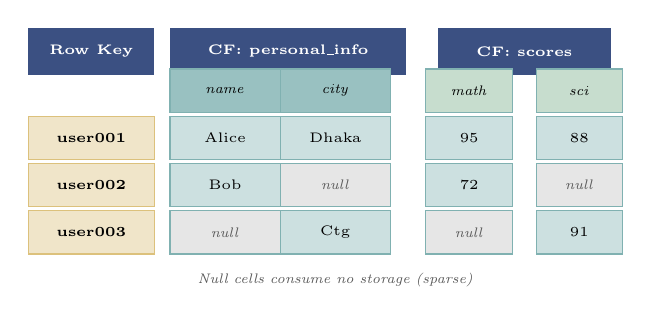
\begin{tikzpicture}[
            hdr/.style={rectangle, fill=PUNavy!80, text=white,
                        minimum height=0.6cm, font=\tiny\bfseries, align=center},
            cf/.style={rectangle, fill=PUTeal!20, draw=PUTeal!50,
                       minimum height=0.55cm, font=\tiny, align=center},
            rk/.style={rectangle, fill=PUGold!25, draw=PUGold!60,
                       minimum height=0.55cm, font=\tiny\bfseries, align=center}
          ]
          % Header row
          \node[hdr, minimum width=1.6cm] (h0) at (0,   3.6) {Row Key};
          \node[hdr, minimum width=3.0cm] (h1) at (2.5, 3.6) {CF: personal\_info};
          \node[hdr, minimum width=2.2cm] (h2) at (5.5, 3.6) {CF: scores};

          % Column headers
          \node[cf, minimum width=1.4cm, fill=PUTeal!40] at (1.7, 3.1) {\textit{name}};
          \node[cf, minimum width=1.4cm, fill=PUTeal!40] at (3.1, 3.1) {\textit{city}};
          \node[cf, minimum width=1.1cm, fill=PUGreen!25] at (4.8, 3.1) {\textit{math}};
          \node[cf, minimum width=1.1cm, fill=PUGreen!25] at (6.2, 3.1) {\textit{sci}};

          % Row 1
          \node[rk, minimum width=1.6cm] at (0, 2.5) {user001};
          \node[cf, minimum width=1.4cm] at (1.7,2.5) {Alice};
          \node[cf, minimum width=1.4cm] at (3.1,2.5) {Dhaka};
          \node[cf, minimum width=1.1cm] at (4.8,2.5) {95};
          \node[cf, minimum width=1.1cm] at (6.2,2.5) {88};

          % Row 2 (sparse)
          \node[rk, minimum width=1.6cm] at (0, 1.9) {user002};
          \node[cf, minimum width=1.4cm] at (1.7,1.9) {Bob};
          \node[cf, minimum width=1.4cm, fill=PUGray!15, text=PUGray]
                at (3.1,1.9) {\textit{null}};
          \node[cf, minimum width=1.1cm] at (4.8,1.9) {72};
          \node[cf, minimum width=1.1cm, fill=PUGray!15, text=PUGray]
                at (6.2,1.9) {\textit{null}};

          % Row 3 (sparse)
          \node[rk, minimum width=1.6cm] at (0, 1.3) {user003};
          \node[cf, minimum width=1.4cm, fill=PUGray!15, text=PUGray]
                at (1.7,1.3) {\textit{null}};
          \node[cf, minimum width=1.4cm] at (3.1,1.3) {Ctg};
          \node[cf, minimum width=1.1cm, fill=PUGray!15, text=PUGray]
                at (4.8,1.3) {\textit{null}};
          \node[cf, minimum width=1.1cm] at (6.2,1.3) {91};

          \node[font=\tiny\itshape, PUGray] at (3.1,0.7)
                {Null cells consume no storage (sparse)};
        \end{tikzpicture}
        \end{center}
      \end{exampleblock}
  \end{columns}
\end{frame}

%----------------------------------------------------------------
\begin{frame}[fragile]{HBase Architecture and Row Key Design}
  \begin{columns}[T]
    \column{0.50\textwidth}
      \begin{block}{HBase Core Components}
        \begin{itemize}
          \item \textbf{HMaster}: coordinates RegionServers; handles schema changes (analogous to NameNode for metadata)
          \item \textbf{RegionServer}: serves reads/writes for a set of \textbf{Regions} (horizontal table partitions by row key range)
          \item \textbf{Region}: contiguous range of rows, stored as \textbf{HFiles} on HDFS
          \item \textbf{ZooKeeper}: distributed coordination; stores HBase master address; detects RegionServer failures
          \item \textbf{WAL (Write-Ahead Log)}: all writes go to WAL on HDFS first, then to in-memory \textbf{MemStore}, then flushed to HFile
        \end{itemize}
      \end{block}
      \vspace{4pt}
      \begin{exampleblock}{Sample HBase Shell Commands}
        \begin{lstlisting}[language={}]
# Create table with two column families
create 'transactions',
  'meta', 'amounts'

# Insert a row
put 'transactions',
  'bkash_20240101_00001',
  'meta:sender', 'user_017'

# Scan a row
get 'transactions',
  'bkash_20240101_00001'
        \end{lstlisting}
      \end{exampleblock}

    \column{0.47\textwidth}
      \begin{alertblock}{Row Key Design: Critical for Performance}
        In HBase, the \textbf{row key determines physical data order}.  Poor key design causes:
        {\small\begin{itemize}
          \item \textbf{Region hotspotting}: sequential keys (e.g., timestamps) send all writes to one Region Server
          \item Solution: \textbf{salt} the key (prepend hash prefix), \textbf{reverse} the timestamp, or use a \textbf{composite key}
        \end{itemize}}
        \vspace{6pt}
        \textbf{Row key examples:}
        \begin{tabular}{ll}
          \toprule
          \textbf{Bad} & \textbf{Good} \\
          \midrule
          \texttt{20240101:user1} & \texttt{7a3b:user1:20240101} \\
          \texttt{20240101:user2} & \texttt{3f1c:user2:20240101} \\
          (hotspot: same Region) & (distributed: hash prefix) \\
          \bottomrule
        \end{tabular}
      \end{alertblock}
      \vspace{4pt}
      \begin{block}{HBase vs.\ HDFS / Hive}
        \small HBase and Hive can \textbf{coexist}: HBase for low-latency operational lookups; Hive for scheduled batch reports over the same underlying HDFS storage.
      \end{block}
  \end{columns}
\end{frame}

%================================================================
\section{Ecosystem Tool Selection}
%================================================================

\begin{frame}{Choosing the Right Tool: Decision Matrix}
  \begin{center}
  \renewcommand{\arraystretch}{1.5}
  \begin{tabular}{p{2.8cm}p{2.3cm}p{2.3cm}p{2.3cm}p{2.3cm}}
    \toprule
    \textbf{Requirement} & \textbf{Raw MapReduce} & \textbf{Pig} & \textbf{Hive} & \textbf{HBase} \\
    \midrule
    Interface language  & Java API        & Pig Latin (script) & HiveQL (SQL) & Java API / Shell \\
    User profile        & Java developer  & Data engineer & SQL analyst  & Java developer \\
    Access pattern      & Sequential batch & Sequential batch & Sequential batch & Random access \\
    Query latency       & Minutes          & Minutes          & Minutes         & Milliseconds \\
    Data structure      & Any              & Semi-structured  & Tabular         & Sparse / wide   \\
    Schema requirement  & None             & Loose            & On-read         & Column families \\
    Write pattern       & Write-once       & Write-once       & Write-once      & Read/write      \\
    Best use case       & Custom algorithm & Complex ETL      & Ad-hoc query    & OLTP on Hadoop  \\
    \midrule
    \textbf{BD example} & Pathao ride logs & bKash ETL        & MOHFW reports   & NID real-time lookup \\
    \bottomrule
  \end{tabular}
  \end{center}
  \vspace{6pt}
  \begin{block}{Key Heuristic}
    Start with \textbf{Hive} if your users know SQL.  Use \textbf{Pig} for multi-step ETL with complex joins.  Use \textbf{HBase} if you need sub-second lookups.  Fall back to raw \textbf{MapReduce} only when the abstraction layers are insufficient.
  \end{block}
\end{frame}

%================================================================
\section{Ivy League Alignment}
%================================================================

\begin{frame}{MapReduce in Top University Curricula}
  \begin{columns}[T]
    \column{0.55\textwidth}
      \begin{block}{Stanford CS246 (Leskovec) — Mining of Massive Datasets}
        \small MapReduce is the \textbf{computational substrate} for the entire course:
        \begin{itemize}
          \item \textbf{Chapter 2}: treats MapReduce as a programming model with specific algebraic properties: \emph{commutativity} and \emph{associativity} are required for Combiners; students prove why average cannot use a Combiner but sum can
          \item \textbf{Cost model}: algorithm analysis uses number of \textbf{reducer inputs} as the primary complexity measure, replacing time complexity — this drives algorithm design
          \item \textbf{Matrix multiplication} and \textbf{graph algorithms} (PageRank) are shown to map onto MapReduce through clever key design
        \end{itemize}
        \textbf{Key exam concept at Stanford:}\\
        \textit{``Design a 2-pass MapReduce algorithm for the join of two 1 TB tables where the join key is uniformly distributed.  Minimise reducer inputs.''}
      \end{block}

    \column{0.42\textwidth}
      \begin{exampleblock}{MIT 6.830 — Database Systems}
        \small MIT compares MapReduce with parallel databases:
        \vspace{4pt}
        \begin{itemize}
          \item DeWitt \& Stonebraker (2008): ``\textit{MapReduce: A major step backwards}'' — critiques lack of schema, indexes, and query optimiser
          \item Pavlo et al. (2009) \textbf{benchmark}: MapReduce vs.\ parallel RDBMS — finds RDBMS 10--100$\times$ faster for structured queries, but MapReduce wins on \textbf{fault tolerance and unstructured data}
        \end{itemize}
        \textit{Hive and Pig were created directly in response to these critiques — adding a query layer and optimiser on top of MapReduce.}
      \end{exampleblock}
      \vspace{4pt}
      \begin{alertblock}{CMU 15-721 — Advanced DB Systems}
        \small CMU frames Hive/HBase as \textbf{competing storage architectures}: row-store (HBase) vs.\ column-store (Parquet/ORC on Hive).  Analytical queries on Hive + ORC approach the performance of dedicated MPP databases for structured data.
      \end{alertblock}
  \end{columns}
\end{frame}

%================================================================
\section{Student Assessment Pool}
%================================================================

\begin{frame}{Assessment\textemdash MCQ Set A \hfill\small\textit{CLO1}}
  \begin{exampleblock}{Instructions}
    Select the single best answer.  Correct answers \textbf{bolded} for instructor reference.
  \end{exampleblock}
  \vspace{8pt}
  \begin{itemize}
    \item[\textbf{Q1.}] In the MapReduce model, which phase sorts and groups intermediate key-value pairs \textbf{before} passing them to Reducers?
    \begin{enumerate}[(a)]
      \item Map \quad (b) \textbf{Shuffle and Sort} \quad (c) Combine \quad (d) Partition
    \end{enumerate}
  \end{itemize}
  \vspace{8pt}
  \begin{itemize}
    \item[\textbf{Q2.}] Which Hadoop ecosystem tool uses a scripting language called \textbf{``Pig Latin''}?
    \begin{enumerate}[(a)]
      \item Hive \quad (b) \textbf{Pig} \quad (c) HBase \quad (d) Sqoop
    \end{enumerate}
  \end{itemize}
  \vspace{8pt}
  \begin{alertblock}{Instructor Notes}
    \textbf{Q1:} Students often confuse \textit{Combine} with \textit{Shuffle and Sort}.  The Combiner is \emph{optional} and runs before shuffle; the Shuffle and Sort phase is \emph{mandatory} and runs as part of the framework — it is what delivers sorted key groups to each Reducer.  \textbf{Q2:} Students sometimes choose Hive because it is more commonly named in general usage.  Reinforce: Hive uses \textbf{HiveQL} (SQL); Pig uses \textbf{Pig Latin} (dataflow scripting).
  \end{alertblock}
\end{frame}

%----------------------------------------------------------------
\begin{frame}{Assessment\textemdash MCQ Set B \hfill\small\textit{CLO1}}
  \vspace{6pt}
  \begin{itemize}
    \item[\textbf{Q3.}] HBase is the open-source implementation of which Google system?
    \begin{enumerate}[(a)]
      \item MapReduce \quad (b) GFS \quad (c) \textbf{Bigtable} \quad (d) Dremel
    \end{enumerate}
  \end{itemize}
  \vspace{8pt}
  \begin{itemize}
    \item[\textbf{Q4.}] Which of the following best describes the HBase data model?
    \begin{enumerate}[(a)]
      \item A relational table with primary and foreign key constraints
      \item A document store where each row contains a JSON blob
      \item \textbf{A sparse, distributed, persistent multidimensional sorted map indexed by row key, column key, and timestamp}
      \item A graph database storing nodes and edges in adjacency lists
    \end{enumerate}
  \end{itemize}
  \vspace{8pt}
  \begin{alertblock}{Instructor Notes}
    \textbf{Q3:} Dremel (option d) is the precursor to Google BigQuery — a common distractor.  The correct mapping is: GFS $\to$ HDFS; Bigtable $\to$ HBase; MapReduce $\to$ MapReduce; Dremel $\to$ BigQuery.  \textbf{Q4:} This quote is taken verbatim from the Bigtable paper (Chang et al., 2006) and is the definition students should memorise.  Option (a) is the most common wrong answer from students familiar only with relational databases.
  \end{alertblock}
\end{frame}

%----------------------------------------------------------------
\begin{frame}{Assessment\textemdash True / False \hfill\small\textit{CLO1}}
  \begin{block}{Instructions}
    State True or False and provide a \textbf{one-sentence justification} for full marks.
  \end{block}
  \vspace{6pt}
  \centering
  \renewcommand{\arraystretch}{1.6}
  \begin{tabular}{p{9.0cm}c}
    \toprule
    \textbf{Statement} & \textbf{Answer} \\
    \midrule
    1.\ MapReduce was originally published by Facebook in 2004. &
    \alert{\textbf{False}} \\
    2.\ Hive queries are compiled at runtime into MapReduce, Tez, or Spark jobs and run on HDFS data. &
    \textbf{True} \\
    3.\ Pig is better suited than Hive for SQL-fluent data analysts who want to write ad-hoc queries. &
    \alert{\textbf{False}} \\
    4.\ HBase supports low-latency random read/write operations, unlike HDFS, which is optimised for sequential reads. &
    \textbf{True} \\
    \bottomrule
  \end{tabular}
  \vspace{6pt}
  \begin{exampleblock}{Model Justifications}
    \small \textbf{1:} MapReduce was published by \textbf{Google} (Dean \& Ghemawat) at OSDI 2004 — Facebook later adopted it and built Hive on top.  \textbf{3:} Pig uses \textbf{Pig Latin}, a procedural dataflow scripting language — it is suited to data engineers, not SQL analysts.  Hive's \textbf{HiveQL} is the SQL-facing interface.
  \end{exampleblock}
\end{frame}

%----------------------------------------------------------------
\begin{frame}{Assessment\textemdash Descriptive Questions \hfill\small\textit{CLO1}}
  \begin{block}{Instructions}
    Answer each question in \textbf{100--150 words}.  Include a diagram where indicated.
  \end{block}
  \vspace{8pt}
  \begin{itemize}
    \item[\textbf{D1.}] Walk through the full MapReduce execution pipeline for the \textbf{word count} problem.  Identify the roles of the Mapper, Combiner, Shuffle/Sort, and Reducer.  Include a \textbf{diagram} showing data flow between these phases.
  \end{itemize}
  \vspace{8pt}
  \begin{itemize}
    \item[\textbf{D2.}] Compare \textbf{Apache Pig} and \textbf{Apache Hive}.  For each tool, state: (a) the language users write in, (b) the programming model (procedural vs.\ declarative), and (c) one type of task it is better suited for.
  \end{itemize}
  \vspace{8pt}
  \begin{itemize}
    \item[\textbf{D3.}] Explain the HBase \textbf{column-family data model}.  How does it differ from a relational schema?  Give a concrete example of a table with two column families and at least two rows, including a \textbf{sparse} row.
  \end{itemize}
\end{frame}

%----------------------------------------------------------------
\begin{frame}{Assessment\textemdash Analytical Questions \hfill\small\textit{CLO1}}
  \begin{block}{Instructions}
    Answer in \textbf{200--300 words} with step-by-step reasoning.  Marks awarded for correct process, not just conclusion.
  \end{block}
  \vspace{6pt}
  \begin{itemize}
    \item[\textbf{A1.}] \textbf{MapReduce Algorithm Design:}\\
    You have a 500 GB log file containing Pathao ride records.  Each record contains: \texttt{(driver\_id, rider\_id, distance\_km, fare\_BDT, timestamp)}.  Design a MapReduce job to find the \textbf{top-10 drivers by total fare earned in January 2024}.
    \begin{itemize}
      \small
      \item Write pseudocode for the Map function (include the filter condition)
      \item Write pseudocode for the Reduce function
      \item Can a Combiner be used?  If yes, write its pseudocode.  If no, explain why.
      \item How would you find the global top-10 if there are 20 Reducer partitions?
    \end{itemize}
  \end{itemize}
  \vspace{6pt}
  \begin{itemize}
    \item[\textbf{A2.}] \textbf{Tool Selection for a Real Scenario:}\\
    A Dhaka-based fintech startup uses HDFS to store 3 years of bKash transaction records (2 TB).  They need: (i) nightly batch reports aggregating total transaction volume by district (SQL-fluent finance team), and (ii) real-time fraud lookups by transaction ID ($<$10 ms response).  Recommend a specific tool for each requirement.  Justify your choices on four dimensions: access pattern, latency, user expertise, and storage model.
  \end{itemize}
\end{frame}

%================================================================
\section*{Textbook References}
%================================================================

\begin{frame}{Textbook \& Reading References}
  \begin{block}{Primary Textbooks for Week 4}
    \begin{itemize}
      \item \textbf{[TW]}\ Tom White. \textit{Hadoop: The Definitive Guide}, O'Reilly, 4th ed., 2015.
            \hfill \textbf{Ch.\ 2, 12, 20}
            \begin{itemize}
              \small\item Ch.\,2: MapReduce · Ch.\,12: Hive · Ch.\,20: HBase
            \end{itemize}
      \item \textbf{[SA]}\ Acharya \& Chellappan. \textit{Big Data and Analytics}, Wiley, 2015.
            \hfill \textbf{Ch.\ 4, 5}
            \begin{itemize}
              \small\item Ch.\,4: MapReduce · Ch.\,5: Pig and Hive
            \end{itemize}
      \item \textbf{[LRU]}\ Leskovec, Rajaraman \& Ullman. \textit{Mining of Massive Datasets}, 3rd ed.
            \hfill \textbf{Ch.\ 2}
            \begin{itemize}
              \small\item Ch.\,2: MapReduce and the New Software Stack (cost model, algorithm design)
            \end{itemize}
    \end{itemize}
  \end{block}
  \vspace{6pt}
  \begin{exampleblock}{Supplementary (Covered in Week 4, Part 2 — Seminal Papers)}
    \begin{itemize}
      \small
      \item Dean, J.\ \& Ghemawat, S.\ (2004). \textbf{MapReduce: Simplified Data Processing on Large Clusters.}
            \textit{OSDI 2004}, pp.\ 137--150.\ \textbf{[PRIMARY SEMINAL PAPER]} ($>$20{,}000 citations)
      \item Chang, F.\ et al.\ (2006). \textbf{Bigtable: A Distributed Storage System for Structured Data.}
            \textit{OSDI 2006}, pp.\ 205--218.\ \textbf{[HBase origin paper]}
      \item Thusoo, A.\ et al.\ (2009). \textbf{Hive — A Warehousing Solution Over a Map-Reduce Framework.}
            \textit{VLDB 2009}.\ \textbf{[Hive origin paper, Facebook]}
    \end{itemize}
  \end{exampleblock}
\end{frame}

%----------------------------------------------------------------
\begin{frame}[c]
  \begin{center}
    {\Large\bfseries Questions \& Discussion}\\[10pt]
    {\large Week 4, Part 1 $\;\mid\;$ CSE 4345 Big Data Analytics}\\[8pt]
    \textcolor{PUGray}{\rule{7cm}{0.5pt}}\\[10pt]
    \begin{quote}
      \itshape ``MapReduce is simple, but its simplicity is deceptive.  The real insight is not the model itself, but the realisation that nearly every large-scale data processing problem can be cast into it.''
    \end{quote}
    \hfill\textemdash\,Jeff Dean, Google (OSDI 2004 presentation)
    \vspace{12pt}
    \begin{block}{\centering Next Lecture: Week 4, Part 2}
      \centering
      Seminal Paper 1: Dean \& Ghemawat (2004) — \textit{``MapReduce: Simplified Data Processing on Large Clusters''}\\[4pt]
      Seminal Paper 2: Chang et al.\ (2006) — \textit{``Bigtable: A Distributed Storage System for Structured Data''}\\[4pt]
      \small Case Study: Facebook's data warehouse migration to Hive (2009) \\
      Scale: 2 PB data · 1{,}000+ engineers · from Java to SQL democratisation
    \end{block}
    \vspace{6pt}
    \textbf{Reading before Part 2:}\ \textbf{[TW]} Ch.\,2 $\cdot$ Dean \& Ghemawat (2004) paper (see references)
  \end{center}
\end{frame}

%=================================================================
\end{document}
%=================================================================
